%% AMS-LaTeX Created with the Wolfram Language for Students - Personal Use Only : www.wolfram.com

\documentclass{article}
\usepackage{amsmath, amssymb, graphics, setspace}

\newcommand{\mathsym}[1]{{}}
\newcommand{\unicode}[1]{{}}

\newcounter{mathematicapage}
\begin{document}

\begin{doublespace}
\noindent\(\pmb{\text{pKlBlei}= \{\{0.41,5.285\},\{0.22,5.859\},\{0.11,6.456\},\{0.058,6.978\},\{0.03,7.422\},\{0.015,7.839\}\};}\\
\pmb{\text{interpolatepKlBlei} = \text{Interpolation}[\text{pKlBlei}];}\\
\pmb{\text{interpolateValue} = \text{interpolatepKlBlei}[0]}\)
\end{doublespace}

\begin{doublespace}
\noindent\(8.43731\)
\end{doublespace}

\begin{doublespace}
\noindent\(\pmb{\text{modellpKlBlei} = \text{Plot}[\text{interpolatepKlBlei}[x],\{x,0,0.45\},\text{PlotRange}\to \{4.5,9\}];}\\
\pmb{\text{graphpKlBlei} = \text{ListPlot}[\text{pKlBlei}];}\\
\pmb{\text{Show}[\text{modellpKlBlei},\text{graphpKlBlei}]}\)
\end{doublespace}

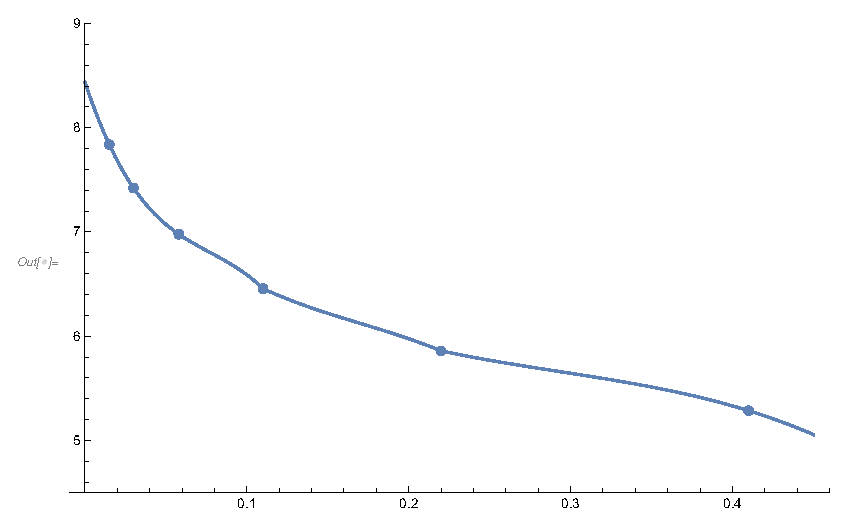
\includegraphics{Auswertung1_gr1.eps}

\end{document}
